\documentclass[tikz,border=2pt]{standalone}
\usepackage{amsmath,amssymb}
\usepackage{tikz}
\usetikzlibrary{arrows.meta}

\begin{document}
% Dropping a constraint enlarges the feasible set: F is contained in F_R, so the relaxed
% optimum is at least as good as the original one (an upper bound for maximisation).
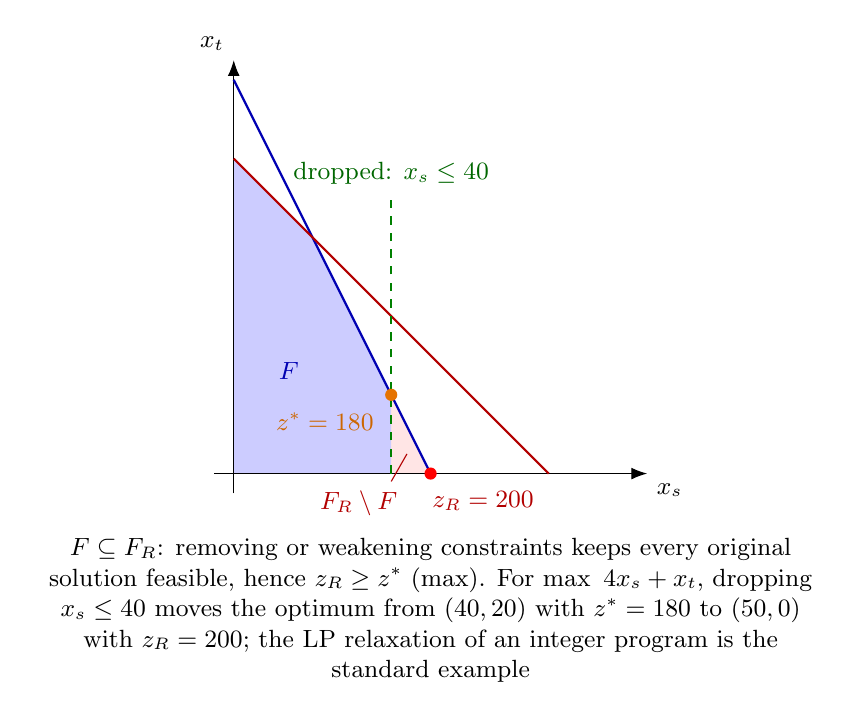
\begin{tikzpicture}[x=0.05cm, y=0.05cm, every node/.style={font=\small}, >={Latex[length=2mm]}]
	\fill[red!10] (0,0) -- (50,0) -- (20,60) -- (0,80) -- cycle;
	\fill[blue!20] (0,0) -- (40,0) -- (40,20) -- (20,60) -- (0,80) -- cycle;
	\draw[->] (-5,0) -- (105,0) node[below right] {$x_s$};
	\draw[->] (0,-5) -- (0,105) node[above left] {$x_t$};
	\draw[blue!70!black, thick] (50,0) -- (0,100);
	\draw[red!70!black, thick] (80,0) -- (0,80);
	\draw[green!50!black, thick, dashed] (40,0) -- (40,70);
	\node[green!40!black, font=\small, anchor=south] at (40,71) {dropped: $x_s\le40$};
	\node[blue!70!black, font=\small] at (14,26) {$F$};
	\draw[red!70!black, thin] (44,5) -- (40,-2);
	\node[red!70!black, font=\small, anchor=north east] at (44,-2) {$F_R\setminus F$};
	\fill[orange!90!black] (40,20) circle (2.2pt);
	\node[orange!80!black, font=\small, anchor=north east] at (38,18) {$z^\ast=180$};
	\fill[red] (50,0) circle (2.2pt);
	\node[red!70!black, font=\small, anchor=north west] at (48,-2) {$z_R=200$};
	\node[anchor=north, align=flush center, text width=10cm] at (50,-14) {$F\subseteq F_R$: removing or weakening constraints keeps every original solution feasible, hence $z_R\ge z^\ast$ (max). For $\max\ 4x_s+x_t$, dropping $x_s\le40$ moves the optimum from $(40,20)$ with $z^\ast=180$ to $(50,0)$ with $z_R=200$; the LP relaxation of an integer program is the standard example};
\end{tikzpicture}
\end{document}
